\documentclass[10pt, twocolumn, a4paper]{article}

\usepackage{microtype}
\usepackage{graphicx}
\usepackage{booktabs} % for professional tables
\usepackage{hyperref}
    \urlstyle{same}
    \hypersetup{colorlinks=true, linkcolor=black, citecolor=black, urlcolor=black}

\usepackage[top=2cm, bottom=2cm, left=1.5cm, right=1.5cm]{geometry}
% \usepackage{fancyhdr}
%     \pagestyle{fancy}
%     \renewcommand{\headrulewidth}{0pt}
\usepackage{titlesec}
    \titleformat{\title}{\large\bfseries}{}{}{}
    \titleformat{\section}{\normalfont\bfseries}{\thesection}{0.5em}{}
    \titleformat{\subsection}{\normalfont\it}{\thesubsection}{0.5em}{}
    \titleformat{\subsubsection}{\normalfont\normalsize\it}{\thesubsubsection}{0.5em}{}
    \titleformat{\paragraph}[runin]{\normalfont\bfseries}{\theparagraph}{0.5em}{}
    \titleformat{\subparagraph}[runin]{\normalfont\normalsize\it}{\thesubparagraph}{0.5em}{}
\usepackage[font=small,labelfont=bf,labelsep=space]{caption}

\usepackage[round]{natbib}
	\renewcommand{\cite}[1]{\citep{#1}}

\usepackage{amsthm, amsmath, amssymb}
\usepackage[ruled]{algorithm2e}
\SetKwComment{Comment}{// }{ }

\usepackage{tikz}
\usetikzlibrary{shapes.geometric, arrows}
\usetikzlibrary{calc}

\tikzstyle{main_node} = [circle, minimum width=1cm,text centered, draw=black, fill=red!30]
\tikzstyle{neigh_node} = [circle, minimum width=1cm,text centered, draw=black, fill=green!30]
\tikzstyle{node} = [circle, minimum width=1cm,text centered, draw=black, fill=cyan!30]
\tikzstyle{arrow} = [thick,->,>=stealth]


\newtheorem{theorem}{Theorem}
\newtheorem{lemma}{Lemma}
\newtheorem{corollary}{Corollary}
\theoremstyle{definition}
\newtheorem{definition}{Definition}

\begin{document}

\author{Oleh Shkalikov (5102818)}
\title{\bf\Large Graph neural networks for solving the multicut problem}
\date{MLCV Seminar, TU Dresden}

\twocolumn[
    \begin{@twocolumnfalse}
        \maketitle

        \vspace{7ex}
    \end{@twocolumnfalse}
]

\section{Summary}

This expository article summarizes the work of \citet{jung2022learning}, focusing on
ways to improve proposed approach which based on heuristics, ideas from
research papers of \citet{chen2019instance} on instance segmentation and self-prior
learning introduced by \citet{Hanocka2020p2m}.

\section{Preliminaries}

The original paper consists of two basic parts: graph neural networks and
minimum cost multicut problem.

\subsection{Graph neural networks}
Graph neural network is a type of neural network which works on arbitrary graphs and can be
described, as it was shown by \citet{gilmer2017neural}, with use of message-passing scheme.

\begin{definition}
    For the given differentiable update function $\gamma:~\mathbb{R}^{d_2} \to \mathbb{R}^{d_3}$,
    differentiable message function $\phi:~\mathbb{R}^{d_1} \times \mathbb{R}^{d_1} (\times \mathbb{R}^{m})~\to~\mathbb{R}^{d_2}$, and
    commutative differentiable aggregation operation $\bigotimes:~\mathbb{R}^{d_2} \times \mathbb{R}^{d_2} \to \mathbb{R}^{d_2}$, the update rule for every
    node $i$ at step $t$ with node feature vector $\mathbf{x} \in \mathbb{R}^{d_1}$ (where $d_{1}$ is a dimensionality
    of the node feature space), neighborhood $\mathcal{N}(i)$ and
    edge feature vector $\mathbf{e} \in \mathbb{R}^m$ (optional, $m$ is a dimensionality of edge feature space) is
    \[
        \mathbf{x}_i^{(t+1)} = \gamma^{(t)} \left(\mathbf{x}_i^{(t)},
        \bigotimes_{j \in \mathcal{N}(i)} \phi^{(t)} \left(\mathbf{x}^{(t)}_i,
        \mathbf{x}^{(t)}_j, \mathbf{e^{(t)}}_{j, i} \right) \right)
    \]
\end{definition}

\begin{figure}[h]
    \centering
    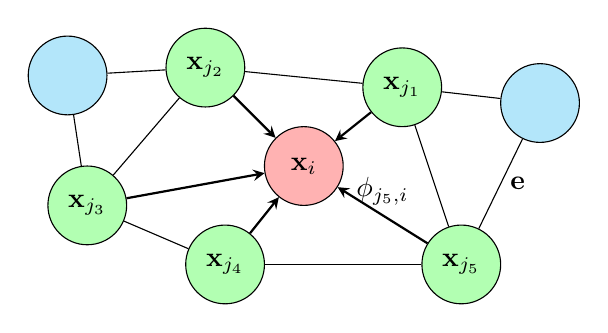
\begin{tikzpicture}[node distance=1.25cm]
        \node(main) [main_node] {$\mathbf{x}_i$};
        \node(neigh1) [neigh_node, right of=main, yshift=1cm] {$\mathbf{x}_{j_1}$};
        \node(neigh2) [neigh_node, left of=main, yshift=1.25cm] {$\mathbf{x}_{j_2}$};
        \node(neigh3) [neigh_node, left of=main, xshift=-1.5cm, yshift=-0.5cm] {$\mathbf{x}_{j_3}$};
        \node(neigh4) [neigh_node, below of=main, xshift=-1cm] {$\mathbf{x}_{j_4}$};
        \node(neigh5) [neigh_node, below of=main, xshift=2cm] {$\mathbf{x}_{j_5}$};

        \node(node1) [node, right of=neigh1, xshift=0.5cm, yshift=-0.2cm] {};
        \node(node2) [node, left of=neigh2, xshift=-0.5cm, yshift=-0.1cm] {};

        \draw[arrow] (neigh1) -- (main);
        \draw[arrow] (neigh2) -- (main);
        \draw[arrow] (neigh3) -- (main);
        \draw[arrow] (neigh4) -- (main);
        \draw[arrow] (neigh5) -- node[above]{$\phi_{j_5, i}$} (main);

        \draw (neigh1) -- (neigh2);
        \draw (neigh1) -- (neigh5);
        \draw (neigh2) -- (neigh3);
        \draw (neigh3) -- (neigh4);
        \draw (neigh4) -- (neigh5);
        \draw (neigh1) -- (node1);
        \draw (neigh5) -- node[right]{$\mathbf{e}$} (node1);
        \draw (neigh2) -- (node2);
        \draw (neigh3) -- (node2);
    \end{tikzpicture}
    \caption{Illustration of the message passing scheme}
\end{figure}

Different graph neural networks architecture can be constructed by specifying all this functions, in
particular the update function, since aggregation operation usually is chosen from the fixed list of
functions such as $\min$, $\max$, mean, sum, product, etc.

Also it is worth to point out, that the graph neural network has a property of locality: the next state of the node depends only on
the current state of the adjacent nodes (and incident edges if they exist), therefore the receptive field
of every node is limited to the number of layers or number of applying the layer to the given graph (usually
on each step different layers are applied).

\subsection{Minimum cost multicut problem}

The minimum cost multicut problem is a combinatorial problem which consists in binary
edge labeling for a given, not necessarily complete, weighted graph. The resulting labeling induced
a partitioning of the graph and can be recognized as an analogue of an instance segmentation for graphs and
that's why has a lot real-world application in computer vision and other fields.

\begin{definition}
    Let $G = (V, E, w)$ be a connected weighted graph, where $V$ is a set of nodes, $E$ -- set of edges and
    $w: E \to \mathbb{R}$ is a weight/cost function. Then the minimum cost multicut
    problem\footnote{The original paper has a typo in the definition of the problem}
    is the following:

    \begin{alignat}{2}
        \min_{y \in \{0, 1\}^E} \quad &
        c(y) = \sum\limits_{e \in E} w_e y_e                                                      \label{def:cost}                  \\
        \text{subject to:}      \quad &
        y_e \leq \sum\limits_{e' \in C \setminus \{e\}} y_{e'}                                         \label{def:cycle_constraint} \\
                                      & \forall C \in \text{cycles}(G), \forall e \in C \nonumber
    \end{alignat}
\end{definition}

The label $1$ means that the corresponding edge is cut.
And the cycle constraints ensure that if the edge was cut then there is no other path in the graph which connects
incident nodes of this edges.

This constraints can be reduced to only chordless cycles as it was shown by \citet{chopra1993partition}, but still for the
non complete graphs (where triangles inequality is sufficient) the constraints grows with size of graph exponentially, so can be
their enumeration can be practically infeasible.

From the point of view of hardness of this integer linear programming problem it is worth to mention that minimum cost multicut
is NP-hard.


\section{Problem statement}

In their article \citet{jung2022learning} address the problem of applying graph neural networks to
the minimum cost multicut problem in order to optimize runtime, but with preserving an
accuracy (in terms of cost) of the solution. And since every neural network consists of
data, architecture, loss function and training process, answering these question is one of the main
task of the paper as well.

\section{Conceptual contributions}

\subsection{General pipeline}

The main conceptual contribution of the paper is a pipeline of applying the graph neural network to
the instance of minimum multicut problem defining by graph. This pipeline can be expressed in the following way.

\begin{algorithm}[h]
    \SetKwInOut{Input}{Input}
    \caption{GNN multicut pipeline}\label{alg:pipeline}
    \Input{$G = (V, E, w)$ -- graph}
    \KwResult{$y \in \{ 0, 1 \}^E$ -- binary labeling of the edges}

    \ForEach{$i \in V$}
    {
        $
            \mathbf{x}_i \gets \left(
            \sum\limits_{j \in \mathcal{N}^{+}(i)} w_{ij},
            \sum\limits_{j \in \mathcal{N}^{-}(i)} w_{ij}
            \right)
        $ \;
        $\mathbf{h_i} \gets \text{GNN}(\mathbf{x_i})$ \;
    }
    \ForEach{$e_{ij} \in E$}
    {
        $y_{ij} \gets \frac{1}{2} \left( \text{MLP} \left( \substack{\mathbf{h_i} \\ \mathbf{h_j}} \right) +
            \text{MLP} \left( \substack{\mathbf{h_j} \\ \mathbf{h_i}} \right) \right) > 0.5$ \;
    }
    Enforce cycle consistency via message passing
\end{algorithm}

Generally, the idea of the approach can be expressed as transforming of the problem of graph partitioning into the real
value clustering problem of node's embeddings, which can be solved by a various methods: in this case with use of MLP.
Then, edges which are incident to the nodes which belong to the different clusters should be cut and
edges which corresponds to the nodes of the same cluster should be preserved.

To perform this transformation from graph to real value node's embeddings an instance of the graph neural
network is being used.

In order to perform the calculation of node embeddings by the message passing approach the input of
graph neural network has to contain initial node features. But since an instance of the minimum cost multicut problem
has only the edge weights authors have proposed the method of computing these features: for each node
they provide 2 dimensional vector where the first component is the sum of all positive incident edge weights and
the second component -- sum of all negative incident edge weights.

Then high dimensional node's embeddings is computed by applying a graph neural network, which will be
discussed in details in the next subsection. The main point to highlight in this regard is that
message passing step  can be run for every node in parallel on GPU which significantly improve runtime of the
full pipeline and which is easy to implement because of existence of a lot deep learning libraries
which provide GPU acceleration out of the box.

On the next step edge classification is performed with use of MLP, i.e. the node's embeddings $\mathbf{h_i}$ and
$\mathbf{h_j}$ of the incident edge $ij$ stacked together in two vectors
$\left( \substack{\mathbf{h_j} \\ \mathbf{h_i}} \right)$ and
$\left( \substack{\mathbf{h_i} \\ \mathbf{h_j}} \right)$. The mean of the MLP with sigmoid head
output is used as a confidence whether an edge should be cut. The final prediction computed by thresholding
this value at $0.5$.

MLP based edge classification requires two vectors because the input graph is considered to be undirected and
MLP is not permutation invariant: the order of inputs
mattes. Also the averaging of the MLP outputs is not so expressible and reliable way to compute the labeling.
The ideas of how to improve this step will be discussed in section \ref{sec:ortho_emb}.

The computed solution can be infeasible since there is no guarantee that cycle consistency \eqref{def:cycle_constraint} won't be
violated. That's why the postprocessing step is required. This step consists in rounding (uncuting wrongly cut edges) of the computed
labeling to enforce the feasibility of the solution. It can be computed by a message passing approach, but since
neither source code nor detailed explanation has been provided by authors we propose our own algorithm \ref{alg:postprocessing}.

\begin{algorithm}[h]
    \SetKwInOut{Input}{Input}
    \caption{Cycle consistency enforcing} \label{alg:postprocessing}
    \Input{$G = (V, E, w)$ -- graph, $y \in \{ 0, 1 \}^E$ -- binary labeling of the edges}
    \KwResult{$\hat{y} \in \{ 0, 1 \}^E$ -- feasible solution}

    \For{$i \in \{1, \dots, |V| \}$}
    {
        $c_i = i$ \Comment{initial class label}
    }

    \For{$n \in \{ 1, \dots, \text{diag}(G) \}$}
    {
        $c \gets \text{MPN}(c)$ \Comment{update rule \eqref{def:postprocessing_mpn}}
    }

    \ForEach{$e_{ij} \in E$}
    {
        $\hat{y}_{ij} \gets c_i = c_j$ \;
    }

\end{algorithm}

For the given graph on the first step for every node we assign different labels which means
that we start with totally separated clusters where only 1 node belong to every particular cluster.
This labels is used as a node's features in the following step.

\begin{figure*}[h]
    \centering
    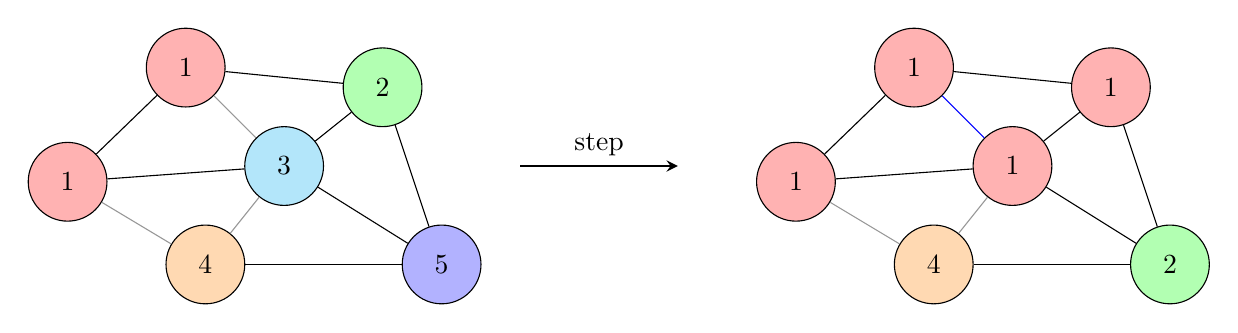
\begin{tikzpicture}[node distance=1.25cm]
        \node(root) [node] {3};
        \node(node1) [node, fill=green!30, right of=root, yshift=1cm] {2};
        \node(node2) [node, fill=red!30, left of=root, yshift=1.25cm] {1};
        \node(node3) [node, fill=red!30, left of=root, xshift=-1.5cm, yshift=-0.2cm] {1};
        \node(node4) [node, fill=orange!30, below of=root, xshift=-1cm] {4};
        \node(node5) [node, fill=blue!30, below of=root, xshift=2cm] {5};

        \node(root2) [node, fill=red!30, right of=root, xshift=8cm] {1};
        \node(node21) [node, fill=red!30, right of=root2, yshift=1cm] {1};
        \node(node22) [node, fill=red!30, left of=root2, yshift=1.25cm] {1};
        \node(node23) [node, fill=red!30, left of=root2, xshift=-1.5cm, yshift=-0.2cm] {1};
        \node(node24) [node, fill=orange!30, below of=root2, xshift=-1cm] {4};
        \node(node25) [node, fill=green!30, below of=root2, xshift=2cm] {2};

        \draw (node1) -- (root);
        \draw[color=gray!80] (node2) -- (root);
        \draw (node3) -- (root);
        \draw[color=gray!80] (node4) -- (root);
        \draw (node5) -- (root);

        \draw (node1) -- (node2);
        \draw (node1) -- (node5);
        \draw (node2) -- (node3);
        \draw[color=gray!80] (node3) -- (node4);
        \draw (node4) -- (node5);

        \draw[arrow] (3, 0) -- node[above]{step} (5, 0);

        \draw (node21) -- (root2);
        \draw[color=blue] (node22) -- (root2);
        \draw (node23) -- (root2);
        \draw[color=gray!80] (node24) -- (root2);
        \draw (node25) -- (root2);

        \draw (node21) -- (node22);
        \draw (node21) -- (node25);
        \draw (node22) -- (node23);
        \draw[color=gray!80] (node23) -- (node24);
        \draw (node24) -- (node25);
    \end{tikzpicture}
    \caption{Illustration of the step of the message passing postprocessing network: colors and labels in nodes corresponds to the
        cluster of nodes: same color and label -- same cluster. Black edges is a uncut edges of the original graph $G$ and
        \textcolor{gray!80}{gray} -- cut edges of $G$. After a message passing step 3 nodes which have been connected by uncut edges
        changed their labels to the minimal label among the neighborhood. At the same time the node with label 4 didn't changed their label
        because it is not connected by uncut edge to any node with smaller label on this step. Also we denote with \textcolor{blue}{blue} color edge that became
        incident to nodes from the same cluster and therefore
        on the last step of the postprocessing algorithm will be restored.} \label{fig:postprocessing}
\end{figure*}

The key component of the postprocessing step is an message passing rule, which is the following:
\begin{equation} \label{def:postprocessing_mpn}
    c_i^{t+1} = \min \left\{ c_i^{t}, \min\limits_{j \in i \cup \mathcal{N}(i)} \left\{ (1 - y_{ij})c_j^{t} + y_{ij} \cdot \infty \right\}  \right\}
\end{equation}
This message passing network on every their step relabel nodes in a way that the resulting label is
equal to the minimum label among the node itself and their adjacent nodes unless adjacent node has been cut.
So, this step is just some variation of a connected component algorithm. But since it is implemented as a message passing
manner it can be parallelized on GPU in the same way as a GNN. But to be sure that we complete finding
all components (merge every component which should be merged for the worst case: linked list) message passing
relabeling has to be run number of steps which is equal to diameter of a given graph (but in real application can
be bounded by a relatively large number or computed precisely if the structure of graph (e.g. grid graph)
is known). The example of the step of a message passing network is given on figure \ref{fig:postprocessing}.

The last step of postprocessing algorithm is responsible for uncut wrongly cut edges by restoring edges
which belongs to the same cluster (that means that there is a path in graph made by uncut edges which
connect this two nodes and therefore constraints \eqref{def:cycle_constraint} have been violated).

\subsection{Graph neural network architectures} \label{sec:architectures}
While all other steps of GNN multicut pipeline \ref{alg:pipeline} don't require
additional changes, architectures of graph neural network should be adjusted to be able to incorporate
edge weights into computation since originally minimum cost multicut problem has only this quantities and
a lot popular models can not work properly without alteration with one dimensional real-valued edge features.

As a main baseline authors of paper have chosen the Graph Convolutional Network by \citet{kipf2016semi}.
The update rule of this architecture is the following:
\[
    \mathbf{x}_i^{(t+1)} = \gamma_{\theta} \left( \mathbf{x}_i^{(t)} +
    \sum\limits_{j \in \mathcal{N}(i)} \mathbf{L_{ij}} \mathbf{x}_j^{(t)} \right),
\]
where update function $\gamma_{\theta}$ is a matrix-vector multiplication with matrix of parameter $\theta$ followed by
non-linear function like ReLU, $\mathbf{L_{ij}} = \frac{1}{\sqrt{\deg(i) \deg(j)}}$ and
$\mathbf{L} = \mathbf{\tilde{D}^{1/2} \tilde{A} \tilde{D}^{1/2}}$ -- normalized graph laplacian, $\tilde{D}$ --
degree matrix and $\tilde{A}$ -- adjacency matrix with additional self-loops.

In order to allow this model to work with negative valued weights (which is necessary because otherwise
the solution is trivial) authors proposed to change the message function by multiplying by weight value and
replacing degree of node with similar but non error-prone quantity
$\overline{\deg}(i) = \sum\limits_{j \in \mathcal{N}(i)} |w_{ij}|$. Thus the update rule of updated
Graph Convolutional Network for minimum cost multicut problem is the following:

\[
    \mathbf{x}_i^{(t+1)} = \gamma_{\theta} \left(
    \mathbf{x^{(t)}_i} +
    \sum_{j \in \mathcal{N}(i)}
    \frac{w_{ij} \mathbf{x}_j^{(t)}}
    {\sqrt{\overline{\deg}(i)} \sqrt{\overline{\deg}(j)}}
    \right)
\]

Despite the fact that all further experiments from the main content of the paper use only this architecture
it is worth to point out that authors also proposed updated version of Signed
Graph Convolutional Network by \citet{derr2018signed} and Graph Isomorphic Network by \citet{xu2018powerful}.
The explanation of choice has not been provided but the given in the appendix graphs allow us to conclude
that decision was based on the stability in terms of training and evaluation loss especially in the case
of Graph Isomorphic Network which has shown big fluctuations. In addition experiments on some
real problems (which will be described further)  have shown that the accuracy of predictions of
Graph Convolutional Network significantly higher than the metric value of all others.

\subsection{Loss function}
Having determined the architecture the next important point in training neural networks and
in particular graph neural network is to define the loss function. In this regard authors decided
to formulate the minimum cost multicut problem as a supervised learning problem with loss which consists of two parts.
They use binary cross entropy loss as the first part of the loss. This part of the loss is responsible for
minimizing the cost \eqref{def:cost} of multicut by making the predicted solution as
close as possible to optimal.

The second part of the loss has been proposed by authors and based on cycle consistency constraints \eqref{def:cycle_constraint}
and responsible for enforcing feasible solutions. They called id CCL (cycle consistency loss) and it is computed as follows:
\begin{equation} \label{eq:ccl}
    \mathcal{L}_{\text{CCL}} = \sum\limits_{C \in cc(G, l)} \sum\limits_{e \in C} \hat{y}_e
    \prod\limits_{e' \in C \setminus \{e\}} (1 - \hat{y}_{e'}),
\end{equation}
where $cc(G, l)$ -- chordless cycles with length less or equal to $l$. This upper boundary is determined
experimentally and necessary since the number of cycles grows exponentially.

The total loss is computed as a weighted sum of these losses. But it worth to point out that supervised
formulation is unnatural for the minimum cost multicut problem and ideas to get rid of this type of
formulation will be discussed in further sections as well as formulation of loss which doesn't require
enumeration of all chordless cycles in the graph.

\subsection{Training process and datasets}
To test their methods authors have trained a lot of networks changing the following parameters:
architectures that we have already discussed in the section \ref{sec:architectures},
with and without using the cycle consistency loss \eqref{eq:ccl}. In addition they varied the architecture
of the Graph Convolutional Network in particular trained the plain (original) model, model
with edge weight but without adding signed normalization term $\left( \overline{\deg}(i) \overline{\deg}(j) \right)^{-\frac{1}{2}}$
and models with both of this addition. They tested different cycle length for the the cycle consistency loss \eqref{eq:ccl},
batch normalization, depth (number of message passing layers) and dimensionality of embeddings.

Since the proposed formulation is a supervised problem, it requires labeled dataset in order to train
GNN and MLP. Despite the fact that the minimum cost multicut problem is widespread number of publicly available
problem instances with provided optimal solutions is limited. To beat this problem the artificially generated
datasets has been created. The final training datasets consists of 2 datasets called IrisMP and RandomMP.

IrisMP datasets consists of minimum cost multicut problem instances defined in a complete graphs and
has been generated based on the well-known Iris flower dataset \citet{fisher1936use} by the
following algorithm: first of all, for each graph only 2 column of the original dataset has been drown
uniformly at random. Then uniformly from 16 to 24 rows has been selected as a nodes and since the graph is complete
all nodes has been connected. Edge weighs have been computed as a output of the logit function applied to
a result of computation of Gaussian kernel with $\sigma = 0.6$ to $L_2$ distances (with respect to the
value of 2 selected from the original Iris dataset columns) between the nodes. In accordance to this
algorithm $20000$ of problem instances has been generated for training and $1000$ graphs for test and
validation splits.

RandomMP dataset contains not complete graphs but with larger number of nodes. The size of this dataset
is equal to the size of IrisMP. To generate this dataset the following algorithm has been used:
the number of nodes for each each graph was sampled from the normal distribution with parameters
$\mu = 180, \sigma = 30$. For each node of the graph its coordinate from $[0, 1]^2$ set has been sampled.
Nodes was connected to the $k$ nearest neighbors, where $k$ was also sampled from the normal distribution with
$\mu = 180, \sigma = 30$ but constrained to be at least $1$. For computing edge weights from the $L_2$ distance
between nodes on the plane the median value of distance has been subtracted in order to end up
with approximately equal number of positive and negative.

It is not clear from the paper how the optimal solutions for these datasets has been computed.
The source code of the paper has not been provided as well. So, with high probability we can consider
that these solutions has been computed with use of some ILP solver (like \citet{gurobi}), since
determining labels based on the generation method (for example determine whether edge between nodes of the graph from IrisMP
dataset should be cut or not based on corresponding flower's species (different species means cut)) may lead to suboptimal solutions.

In addition, it is worth to mention that problem instances from artificially generated datasets can
significantly differ from the real-world problem instances which can lead to lower performance of the model
trained on this data. But with use of this approach authors could generate sufficiently large
dataset for training neural networks.

As a metric for the evaluation authors proposed the optimal objective ratio:
\[
    m = \max \left\{ 0, \frac{c(\hat{y})}{c(\tilde{y})} \right\},
\]
where $c$ is a an objective or cost \eqref{def:cost}, $\hat{y}$ -- predicted solution,
$\tilde{y}$ -- optimal solution. This metric is computed on postprocessed output of the
pipeline \ref{alg:pipeline} and can be considered as better than classical classification
metrics like F1, precision and recall since the main objective of the optimization task is to
minimize the total cost and therefore incorrect predictions of edge labels has different impact (higher absolute value
of the weight -- higher impact) to the cost whereas classical metrics considered this impact as
equal for all edges.

\section{Empirical contributions} \label{sec:empirical_contib}

For the evaluation in addition to generated instances of problem authors used
dataset \citet{andres2011probabilistic} based on the Berkeley Segmentation Dataset (BSDS300) \citet{martin2001database},
volume segmentation dataset Knott3D \citet{andres2012globally} and
Circuit Reconstruction from Electron Microscopy Images (CREMI) \citet{beier2017multicut}.
The proposed approach has been compared to exact ILP solver as well as Branch \& Cut LP (\citet{kappes2015comparative})
and GAEC (\citet{keuper2015efficient}) (time-bounded and not).

The main results of the experiment can be summarized as follows: the GNN pipeline \ref{alg:pipeline}
is the best solver in the context of trade-off between runtime and resulting cost of multicut. Whereas
classical methods show better objective value, the GNN (in particular proposed GCN architecture)
significantly faster and computed solution is comparable to the competitors. Time bounded GAEC in comparison
to the discussed approach is tremendously worse. These results preserves with growing of the size of
input problem instance.

Ablation study proves the efficiency of proposed cycle consistency loss \eqref{eq:ccl} and changes committed to
the GNN architecture. Additionally, authors denoted examples where for the particular instances of problem
GNN generated embeddings for nodes such that their cosine similarities reflects the resulting cluster.

\section{Ideas to improve the proposed approach}
The proposed approach can be possibly improved by using additional heuristics,
ideas from other methods and by analyzing the experimental result. In this section
we will offer some ideas of how to do it.

\begin{figure*}[t]
    \centering
    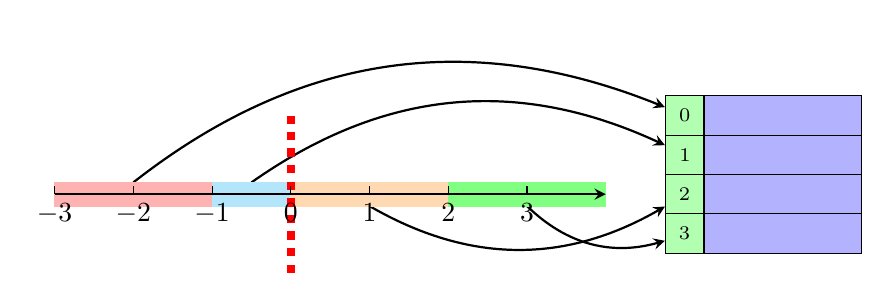
\begin{tikzpicture}
        \tikzstyle{emb_bin} = [draw, fill=green!30, text centered, text width=0.25cm, font=\scriptsize, minimum height=0.5cm]
        \tikzstyle{emb} = [draw, fill=blue!30, minimum width=2cm,minimum height=0.5cm]

        \node (bin0) at (5, 1) [emb_bin] {0};
        \node [emb, right of=bin0, xshift=0.25cm] {};
        \node (bin1) at (5, 0.5) [emb_bin] {1};
        \node [emb, right of=bin1, xshift=0.25cm] {};
        \node (bin2) at (5, 0) [emb_bin] {2};
        \node [emb, right of=bin2, xshift=0.25cm] {};
        \node (bin3) at (5, -0.5) [emb_bin] {3};
        \node [emb, right of=bin3, xshift=0.25cm] {};

        \draw[arrow] (-2, 0.15)   to[bend left] (bin0);
        \draw[arrow] (-0.5, 0.15) to[bend left] (bin1);
        \draw[arrow] (1, -0.15)   to[bend right] (bin2);
        \draw[arrow] (3, -0.15)   to[bend right] (bin3);

        \draw[color=red!30, fill=red!30] (-3,-0.15) rectangle ++(2, 0.3);
        \draw[color=cyan!30, fill=cyan!30] (-1,-0.15) rectangle ++(1, 0.3);
        \draw[color=orange!30, fill=orange!30] (0,-0.15) rectangle ++(2, 0.3);
        \draw[color=green!50, fill=green!50] (2,-0.15) rectangle ++(2, 0.3);

        \draw[color=red, dashed, line width=0.1cm] (0,-1) -- (0, 1);

        \draw[arrow] (-3,0) -- (4,0);
        \foreach \x in {-3,-2,...,3}{
                \draw (\x, 0.1) -- (\x,0) node[below]{$\x$};
            }
    \end{tikzpicture}
    \caption{Illustration of assigning embeddings to bins of weight's value}
    \label{fig:edge_embeddings}
\end{figure*}

\subsection{Orthogonal embeddings} \label{sec:ortho_emb}
As it has been discussed in section \ref{sec:empirical_contib}, it is possible for model
to produce node's embeddings for which cosine similarities will be enough to decide whether
edge should be cut or not. The idea is to train a model explicitly to produce such embeddings.
But since usual cosine similarities has 3 key values which corresponds to 3 "states":
similar (value close to $1$), orthogonal (value close to $0$) and opposite (value close to $-1$), -
whereas the labeling of edges (node pairs) has 2 states: uncut (nodes belong to the same cluster) and cut
(nodes belongs to the opposite cluster) we propose to use the following quantity from the paper
of \citet{chen2019instance}:
\begin{equation} \label{eq:ortho_sim}
    1 - |\cos \langle \mathbf{x}_i, \mathbf{x}_j \rangle|
\end{equation}

By thresholding quantity \eqref{eq:ortho_sim} with some number $t \in [0, 0.5]$ we label edges between nodes
in a way that adjacent nodes with collinear embeddings will belong to the same component (edge is not cut)
and with orthogonal -- to different components (edge is cut). And as it has been shown in the
paper we don't need to care (if we chose sufficiently large embedding's dimensionality)
about situation when non adjacent has collinear embeddings and utilize only local orthogonality.

The loss function which can help us to learn it is similar to the loss from \citet{chen2019instance} as well:
\begin{align} \label{eq:ortho_loss}
    \mathcal{L}_{emb} =
     & \lambda_1 \sum\limits_{e_{ij} \in y^{-1}(0)} \left(1 - |\cos \langle \mathbf{x}_i, \mathbf{x}_j \rangle| \right) + \\
     & \lambda_2 \sum\limits_{e_{ij} \in y^{-1}(1)} |\cos \langle \mathbf{x}_i, \mathbf{x}_j \rangle|,
\end{align}
where $\lambda_1, \lambda_2$ -- some normalization weights which depends on the number of cut and non cut edges.

Unfortunately, this approach can not enforce cycle consistency in a transitive manner
(suppose $t < 0.5$)
\begin{multline*}
    \begin{cases}
        1 - |\cos \langle \mathbf{x}_i, \mathbf{x}_j \rangle| \leq t \\
        1 - |\cos \langle \mathbf{x}_j, \mathbf{x}_k \rangle| \leq t
    \end{cases} \implies \\
    1 - |\cos \langle \mathbf{x}_i, \mathbf{x}_k \rangle| \leq
    1 - |2(1 - t)^2 - 1| \geq t
\end{multline*}

As a result, this approach allow us to get rid of MLP classifier on the head of the GNN and give a
meaningful explanation of node embeddings and edge classification / labeling.

\subsection{Relaxed Cycle Consistency Loss}
The existing cycle consistency loss \eqref{eq:ccl} requires enumeration of all
chordless cycles of length $\leq l$ which can lead to enormous number of cycles since
their number grows exponentially.

In the same time it has been shown by authors that increasing length of cycles
doesn't improve the quality of the model. This explained by the fact that in a process of calculation
we multiply a lot number in range $[0, 1]$. And whereas the problem of machine zero can be solved by
exp-sum-log trick, the conceptual problem, that for large $l$ the loss value will be very small and
therefore impact of this wrong prediction is imperceptible, still exists.

To handle thess issues we propose the following relaxed cycle consistency loss:
\[
    \frac{1}{|E|} \sum\limits_{e \in \tilde{E}} \hat{y}_e,
\]
where $\tilde{E}$ -- set of all cut edges which violate cycle consistency constraint \eqref{def:cycle_constraint}.

This loss doesn't require enumeration of cycles as well as doesn't suffer from the problem of
multiplication of small numbers. But on the other hand loss will be "backpropagated" only to the
wrongly cut edges where the original loss penalties all edges within the cycle for which constraint
has been violated.

\subsection{Edge Weight Embedding}

There are a lot of GNN architectures (e.g. Graph Attention Network \citet{velickovic2017graph} )
that work with edge attributes. But attributes should be high dimensional (since multiplication of
weight by some shared parameter doesn't change anything).
The idea of edge weight embedding is to split weights into
bins (ranges) and then assign for every bin learnable embedding
(similar to assigning embedding to token in NLP).

The important point in this regard is that negative and positive values always should belong
to different bins. The figure \ref{fig:edge_embeddings} shows
the idea of the method.

This idea is the most controversial and there is no even hypothetical clue that it can improve
the performance of the model.

\subsection{Unsupervised formulation}
The original formulation of the problem is supervised which requires having
an labeled dataset for training. But in their nature minimum cost multicut problem is an
unsupervised problem. But the only thing which make the current formulation supervised is
a binary cross-entropy loss (even orthogonal loss \eqref{eq:ortho_loss} doesn't depend on optimal solution).

We can try replace $\mathcal{L}_{BCE}$ loss with
loss which depends on the cost of cut \eqref{def:cost} itself. For example, let $\beta_t$ be
a decreasing sequence, then multicut cost loss can be as follows:
\[
    \mathcal{L}_{MC}^{t} (\hat{y}) = \beta_t \left( c(\hat{y}) - c_{LB} \right),
\]
where $c_{LB} = \sum\limits_{w_i < 0} w_i$ -- a lower bound of the cost.

It is supposed that on the first steps of training, when $\beta$ is high, our model will learn to
assign the minimum possible cost and then, when $\beta$ become small we will take care of the cycle
consistency \eqref{def:cycle_constraint} and other losses.

Moreover, from some point of view this loss is more natural for the given multicut problem since
classical cross-entropy doesn't distinguish between incorrect labeling of the edge with
small and big absolute value, whereas the impact on the cost (which we actually try to minimize)
is not equal for different weight's values. And the proposed formulation considers these different impacts.

\subsection{Self-prior learning / finetuning}
Learning on large datasets allow model generalize
based on data instead of overfit,
but with the generalization model can defeat on particular examples.
But our task is to assign the best possible costs for all problems and
initially we don't need generalization property.

Unsupervised formulation allow us to perform self-prior~(inspired by \citet{Hanocka2020p2m})
learning: overfit different, possibly graph depended model (e.g. vary
number of layers w.r.t. the size of graph) on every particular graph which
can allow model to output the best result for this specific instance of minimum cost multicut problem.

In this of course we have to retrain model for every
graph and it requires time (which is the main advantages of the GNN pipeline).
It is not just an simple inference as it was in the previous cases, but it can be
relaxed if the "training" process will start from already pretrained
network (overfitting by finetuning).

\bibliography{../references.bib}
\bibliographystyle{plainnat}

\end{document}

